\documentclass[12pt,compress,aspectratio=169]{beamer}
\usetheme{metropolis}
\setbeamersize{text margin left=.5cm,text margin right=.5cm}
\usepackage[lf]{carlito}
\usepackage{tikz}
\usepackage{mathpazo}
\usepackage{xcolor,colortbl}
\usepackage{siunitx}
\setlength{\parskip}{0pt}
\renewcommand{\baselinestretch}{1}
\sisetup{
  inter-unit-product=\cdot,
  per-mode=symbol
}
\tikzset{>=latex}

\title{Topic 18: Special Relativity}
\subtitle{AP and IBHL Physics}
\author[TML]{Dr.\ Timothy Leung}
\institute{Olympiads School}
\date{\today}



\newcommand{\mb}[1]{\mathbf{#1}}
\newcommand{\pic}[2]{\includegraphics[width=#1\textwidth]{#2}}
\newcommand{\bigsqrt}{\ensuremath\sqrt{1-\left(\frac{v}{c}\right)^2}}
\newcommand{\lorentz}{\ensuremath\frac{1}{\bigsqrt}}
\newcommand{\eq}[2]{\vspace{#1}{\Large\begin{displaymath}#2\end{displaymath}}}



\begin{document}

\begin{frame}
  \maketitle
\end{frame}



\section{Simultaneity}

\begin{frame}{The Relativity of Simultaneity}
  This \emph{thought experiment} is similar to the one that Einstein presented.
  Suppose lightning bolt strikes the two ends of a high-speed moving train.
  Does it happen simultaneously?
  \begin{center}
    \pic{.4}{graphics/87-1-1024x673.png}
  \end{center}

  \begin{itemize}
  \item\vspace{-.15in} Two \emph{independent} events: lightning striking the
    front, and lightning striking the back of the train
  \item The man on the ground sees the lightning bolt striking at the same time
  \item The woman on the moving train sees the lightning bolt on the front first
  \end{itemize}
\end{frame}



\begin{frame}{Relativity of Simultaneity}
  From the man's perspective:
  \begin{itemize}
  \item He is stationary, but the train is moving
  \item When the lightnings strike, he is at an equal distance from the front
    and the back of the train
  \item Flashes from the two lightning bolts arrive at his eyes at the same time
  \item Since the speed of light is a constant regardless of motion
  \end{itemize}
  Therefore, his conclusions are:
  \begin{itemize}
  \item The two lightnings must have happened at the same time
  \item The woman in the train made the wrong observation: she only
    \emph{thinks} that the lightning struck the front first because she is
    moving toward the light from the front
  \end{itemize}
\end{frame}


\begin{frame}{Relativity of Simultaneity}
  From the woman's perspective:
  \begin{itemize}
  \item\emph{She} is stationary, but the man and the rest of the world are
    moving
  \item When the lightnings strike, she is at an equal distance from the two
    ends of the train
  \item The flash from the front arrive first, then the back
  \item Since the speed of light is a constant regardless of motion
  \end{itemize}
  Therefore, her conclusions are:
  \begin{itemize}
  \item Lightnings must have struck the front first
  \item The man on the road made the wrong observation: he only \emph{thinks}
    that the lightning struck at the same time because he's moving toward the
    light from the back
  \end{itemize}
\end{frame}


\begin{frame}{Relativity of Simultaneity}
  \begin{itemize}
  \item The two observers disagree on the result, but
    \begin{itemize}
    \item Neither person is wrong
    \item Neither person is misinformed
    \end{itemize}
  \item Both observers are valid \emph{inertial} frames of reference, and
    therefore both can consider themselves at rest
  \item This means that \emph{simultaneity depends on your motion}
  \end{itemize}
  
  \vspace{.2in}\textbf{Relativity of Simultaneity: Events that are simultaneous
    in one inertial frame of reference are not simultaneous in another.}
\end{frame}



\section{Time Dilation}


\begin{frame}{Relativity of Time: Time Dilation}
  \begin{center}
    \pic{.25}{graphics/spaceship1}
  \end{center}
  \vspace{-.15in}I'm on a spaceship travelling in deep space, and I shine a
  light from $A$ to $B$. The distance between $A$ and $B$ is:

  \eq{-.3in}{
    |AB|=c\Delta t_0
  }

  \vspace{-.1in}I know the speed of light $c$, and I know how long it took for
  the light pulse to reach $B$. (The reason I used $\Delta t_0$ will be obvious
  later.)
\end{frame}


\begin{frame}{Relativity of Time: Time Dilation}
  \begin{center}
    \pic{.55}{graphics/spaceship2}
  \end{center}
  You are on a small planet watching my spaceship go past you at speed $v$. You
  would see that same beam of light travel from $A$ to $B'$ instead.
\end{frame}



\begin{frame}{Relativity of Time: Time Dilation}
  We can relate the time interval observed by me on the spaceship ($t$) and
  your time interval on the small planet ($t'$) using Pythagorean theorem:
  \begin{columns}
    \column{.35\textwidth}
    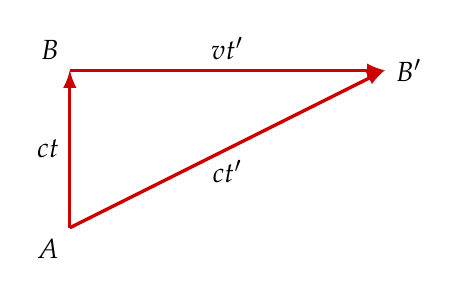
\begin{tikzpicture}
      \draw[very thick,red!80!black,->](0,0)--(0,2)
      node[pos=0, below left,black]{$A$}
      node[midway,left,black]{$ct$}
      node[above left,black] {$B$};
      \draw[very thick,red!80!black,->](0,2)--(4,2)
      node[midway,above,black]{$vt'$} node[right,black]{$B'$};
      \draw[very thick,red!80!black,->](0,0)--(4,2)
      node[midway,below, black]{$ct'$};
    \end{tikzpicture}
    
    \column{.6\textwidth}
    \begin{align*}
      (ct')^2 &=(vt')^2 + (ct)^2\\
      \left(c^2-v^2\right)t'^2 &=c^2t^2\\
      \left(1-\frac{v^2}{c^2}\right)t'^2 &=t^2\\
      t' &=\frac{t}\bigsqrt
    \end{align*}
  \end{columns}
  \vspace{.1in}\textbf{Relativity of time}: the passage of time as measured by
  two observers in two different inertial references are different
\end{frame}



\begin{frame}{Relativity of Time: Time Dilation}
  The passage of time as measured by two observers in two different inertial
  frames of reference are related by:
  
  \eq{-.2in}{
    \boxed{t' =\frac{t}\bigsqrt}
  }
  \begin{center}
    \begin{tabular}{l|c|c}
      \rowcolor{pink}
      \textbf{Variable} & \textbf{Symbol} & \textbf{SI Unit}\\ \hline
      Proper time (ordinary time)  & $t$  & \si{\second} \\
      Dilated time (expanded time) & $t'$ & \si{\second} \\
      Speed           & $v$ & \si{\metre\per\second}\\
      Speed of light  & $c$ & \si{\metre\per\second}
    \end{tabular}
  \end{center}
  \begin{itemize}    
  \item\textbf{Proper time} is measured by an observer \emph{at rest} relative
    to the events
  \item\textbf{Dilated time} is measured by a \emph{moving} observer in another
    inertial frame
  \end{itemize}
\end{frame}



\begin{frame}{Example Problem}
  \textbf{Example 1a:} Kim is riding a rocket that speeds past an asteroid at
  $v=0.600c$. If Kim sees \SI{10.}{\second} pass on her watch, how long would
  that time interval be as seen by Jim, an observer on the asteroid?

  \uncover<2>{
    \begin{displaymath}
      t' =\frac{t}\bigsqrt=\frac{10.}{\sqrt{1-0.600^2}}=\SI{16.7}{\second}
    \end{displaymath}
  }
  
  \uncover<3>{
    \begin{itemize}
    \item Jim observes that in the time it took Kim's clock to run
      \SI{10.}{\second}, his watch has already gone \SI{16.7}{\second},
      therefore
    \item Jim concludes that Kim's watch must be running slow
    \end{itemize}

    \textbf{Relativity of Time: A moving clock appears to run slow.}
  }
\end{frame}



\begin{frame}{Example Problem}
  \textbf{Example 1b:} Kim is riding a rocket that speeds past an asteroid at
  $0.600c$. If Jim, an observer in the \emph{asteroid}, sees \SI{10.}{\second}
  pass on his watch, how long would that time interval be as seen by Kim?

  \uncover<2>{
    \begin{displaymath}
      t' =\frac{t}\bigsqrt=\frac{10.}{\sqrt{1-0.600^2}}=\SI{16.7}{\second}
    \end{displaymath}
    
    \begin{itemize}
    \item This problem is exactly the same as the last one!
    \item Kim observes that in the time it took Jim's clock to run
      \SI{10.}{\second}, her watch has already gone \SI{16.7}{\second},
      therefore
    \item Kim concludes that Jim's watch must be running slow
    \end{itemize}
  }
\end{frame}



\begin{frame}{How can that be?}
  How can the observer in the asteroid sees time in the rocket runs slowly,
  while the observer in the rocket \emph{also} sees time in the asteroid runs
  slowly?

  \vspace{.3in}\textbf{Answer:} the relativty of simultaneity. The clocks on the
  asteroid and on the rocket are \emph{not} synchronized.
  \begin{itemize}
  \item In example 1a, when Kim (on the rocket) starts measuring a
    \SI{10.}{\second} time interval, in order for Jim to compare that interval
    to \emph{his} watch, he has to start and end at the same time
    (simultaeously!) as Kim.
  \item But simultaneity is only relative. In Kim's reference frame, Jim never
    got the timing right!
  \item This problem reverses itself when Kim tries to synchronize her watch to
    Jim's \SI{10.}{\second} interval.
  \end{itemize}
\end{frame}


\section{Length Contraction}

\begin{frame}{Relativity of Space}
  Captain Quick is a comic book hero who can run at nearly the speed of light.
  In his hand, he is carrying a bomb set to explode in \SI{1.5}{\micro\second}.
  The bomb must be placed into its bracket before this happens. The distance
  ($L$) between the flare and the bracket is \SI{402}{\metre}.
  \begin{center}
    \pic{.7}{graphics/captain-quick}
  \end{center}
\end{frame}


\begin{frame}{Relativity of Space}
  Suppose Captain Quick runs at \SI{2.00e8}{\metre\per\second}, according to
  classical mechanics, he will not make it in time:
  \begin{displaymath}
    t= \frac{L}{v}=\frac{\SI{402}{\metre}}{\SI{2.00e8}{\metre\per\second}}
    =\SI{2.01e-6}{\second}=\SI{2.01}{\micro\second}
  \end{displaymath}
  But according to relativistic mechanics, he makes it just in time\ldots
\end{frame}


\begin{frame}{Relativity of Space}
  To a stationary observer, the time on the flare is slowed:
  \begin{displaymath}
    t'
    = \frac{t}{\bigsqrt}
    = \frac{\num{1.5e-6}}{\sqrt{1-\left(\frac{2.00}{3.00}\right)^2}}
    = \SI{2.01e-6}{\second}
  \end{displaymath}
  The stationary observer sees a passage of time of
  $t'=\SI{2.01}{\micro\second}$, but Captain Quick, who is in the same
  reference frame as the flare, experiences a passage of time of
  $t=\SI{1.50}{\micro\second}$, precisely the time for the flare to explode.
\end{frame}


\begin{frame}{Relativity of Space}
  If Captain Quick sees only $t=\SI{1.50}{\micro\second}$, then how far did he
  travel?
  \begin{itemize}
  \item Both Captain Quick and the observer on the side of the road agree that
    he is traveling at $v=\SI{2.00e8}{\metre\per\second}$
  \item The only possibility is that \emph{the distance actually got shorter}
    in Captain Quick's frame of reference, by this amount:
    
    \eq{-.2in}{
      \boxed{L'=L\bigsqrt}
    }
  \end{itemize}
  For this example:
  \begin{displaymath}
    L'=L\bigsqrt=402\sqrt{1-\left(\frac{2.00}{3.00}\right)^2}=\SI{300}{\metre}
  \end{displaymath}
\end{frame}



\begin{frame}{Length Contraction}
  Length contraction only occurs in the direction of motion
  \begin{center}
    \pic{.8}{graphics/baseball-contraction}
    \end{center}
\end{frame}



\begin{frame}{Example Problem}
  \textbf{Example 2:} A spacecraft passes Earth at a speed of \SI{2.00e8}{m/s}.
  If observers on Earth measure the length of the spacecraft to be
  \SI{554}{\metre}, how long would it be according to its passengers?
\end{frame}


\section{Lorentz Factor}

\begin{frame}{Lorentz Factor}
  The \textbf{Lorentz factor} $\gamma$ is a short-hand for writing length
  contraction, time dilation and relativistic mass:

  \eq{-.2in}{
    \boxed{\gamma=\lorentz}
  }
  
  Then time dilation and length contraction can be written simply as:
  
  \eq{-.1in}{
    \boxed{t' = \gamma t}\quad\boxed{L' = \frac{L}{\gamma}}
  }
\end{frame}



\begin{frame}{Summary}
  \begin{center}
    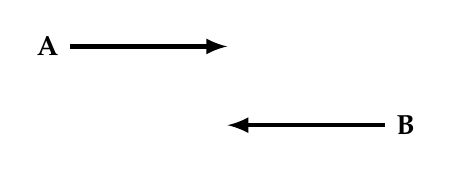
\begin{tikzpicture}[scale=2]
      \draw[ultra thick,->] (1,.5)--(2,.5) node[pos=0,left] {\textbf{A}};
      \draw[ultra thick,->] (3,0)--(2,0) node[pos=0,right]{\textbf{B}};
    \end{tikzpicture}
  \end{center}
  If observers A and B are moving at constant velocity relative to one another
  (doesn't matter if they're moving toward, or away from each other)
  \begin{itemize}
  \item They cannot agree whether any events happens at the same time or not
  \item Each sees the other's clock running slow
  \item Each sees the other ``contracted'' in length along the direction of
    motion
  \end{itemize}
\end{frame}


\begin{frame}{Lorentz Transformation}
  Time dilation and length contraction only tell part of the story. To account
  for the loss of simultaneity from one inertial frame to another, we need to
  use the \textbf{Lorentz transformation:}

  \vspace{-.45in}{\Large
    \begin{align*}
      x' &= \gamma(x-vt)\\
      y' &= y\\
      z' &= z\\
      t' &=\gamma\left(t-\frac{vx}{c^2}\right)
    \end{align*}
  }
  
  \vspace{-.1in}The Lorentz transformation ``solves'' many paradoxes
  (e.g.\ the twin paradox) from the time-dilation and
  length-contraction equations, but aren't really there.
\end{frame}



\begin{frame}{Lorentz Transformation}
  For slow speeds $v\ll c$, Lorentz transformation reduces to the Galilean
  transformation from classical mechanics, from which the velocity addition
  rule is formulated:

  \vspace{-.45in}{\Large
    \begin{align*}
      x' &= x-vt\\
      y' &= y\\
      z' &= z\\
      t' &= t'
    \end{align*}
  }
\end{frame}



\section{Relative Velocity}

\begin{frame}{Relative Velocity}
  Unlike in classical mechanics, velocities (speeds) do not simply add. We have
  to account for time dilation and length contraction, which are included in
  the Lorentz transformation

  \vspace{.15in}\textbf{Einstein velocity addition rule}:

  \eq{-.2in}{
    \boxed{
      \mb{v}_{AC}=
      \frac{\mb{v}_{AB}+\mb{v}_{BC}}
           {1+\frac{\mb{v}_{AB}\cdot\mb{v}_{BC}}{c^2}}
    }
  }

  \vspace{.1in} If $v_{AB}\ll c$ and $v_{BC}\ll c$, we recover Galilean
  velocity addition rule
\end{frame}
\end{document}
